\chapter{Long baseline water Cherenkov detectors}
\label{chap:wc}

%%%%%%%%%%%%%%%%%%%%%%%%%%%%%%%%%%%%%%%%%%%%%%%%%%%%%%%%%%%%%%%%%%%%%%%%%%%%%%%%%%%%%%%%%%%%%%%%%%
%                                              PLAN                                              %
%%%%%%%%%%%%%%%%%%%%%%%%%%%%%%%%%%%%%%%%%%%%%%%%%%%%%%%%%%%%%%%%%%%%%%%%%%%%%%%%%%%%%%%%%%%%%%%%%%
\begin{comment}
TODO: Write the story of the wc chapter

TODO: Write the wc chapter section outline

NEUTRINO INTERACTIONS
- Feynman diagrams of all the main interaction types
- Famous diagrams of cross-section regions for them all
- Descriptions of which types are easy to detect, what are the main NC backgrounds usually etc...

\end{comment}

- Say how they are usually very expensive due to volume required
- Large overburden/excavation costs etc...
- Beam
- cherenkov light
- PMTs
- water clarity
- overburden
- interaction types (which ones are the problem)
- What they are good at, what they are bad At
- Historical WC detectors

%%%%%%%%%%%%%%%%%%%%%%%%%%%%%%%%%%%%%%%%%%%%%%%%%%%%%%%%%%%%%%%%%%%%%%%%%%%%%%%%%%%%%%%%%%%%%%%%%%
%                                     NEUTRINO INTERACTIONS                                      %
%%%%%%%%%%%%%%%%%%%%%%%%%%%%%%%%%%%%%%%%%%%%%%%%%%%%%%%%%%%%%%%%%%%%%%%%%%%%%%%%%%%%%%%%%%%%%%%%%%
\section{Neutrino interactions}
\label{sec:theory_interactions}

\begin{figure} % CROSS-SECTION DIAGRAM %%%%%%%%%%%%%%%%%%%%%%%%%%%%%%%%%%%%%%%%%%%%%%%%%%%%%%%%%%%
    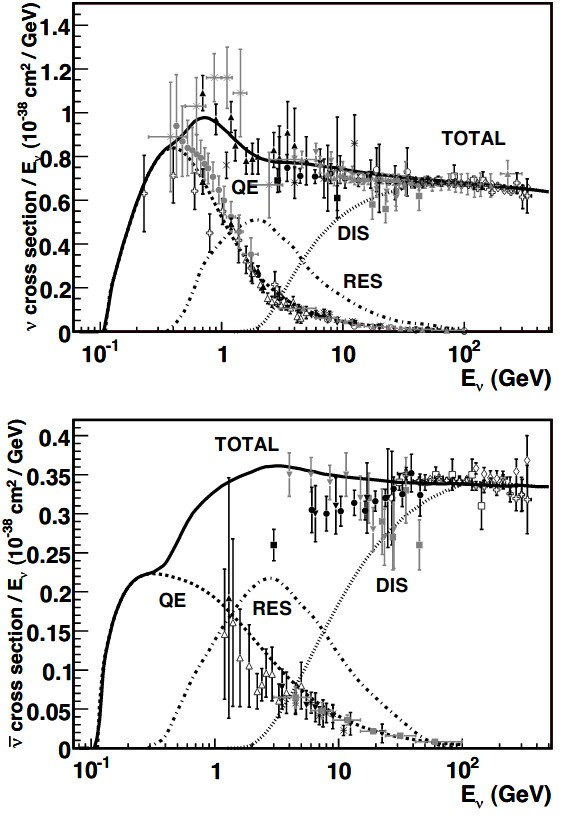
\includegraphics[origin=c,width=0.6\textwidth]{diagrams/4-wc/cross_sections.png}
    \caption[cross sections short]
    {Figure taken from Ref.\cite{formaggio2012}.}
    \label{fig:cross_sections}
\end{figure} %%%%%%%%%%%%%%%%%%%%%%%%%%%%%%%%%%%%%%%%%%%%%%%%%%%%%%%%%%%%%%%%%%%%%%%%%%%%%%%%%%%%%

\begin{figure} % TAU CROSS-SECTION DIAGRAM %%%%%%%%%%%%%%%%%%%%%%%%%%%%%%%%%%%%%%%%%%%%%%%%%%%%%%%
    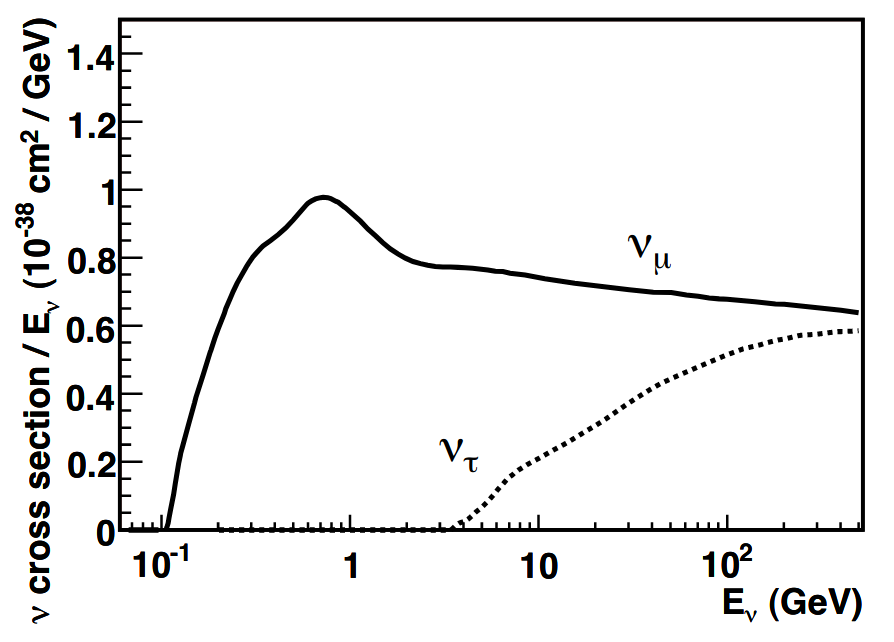
\includegraphics[origin=c,width=0.6\textwidth]{diagrams/4-wc/tau_comparison.png}
    \caption[tau comparison short]
    {Figure taken from Ref.\cite{formaggio2012}.}
    \label{fig:tau_comparison}
\end{figure} %%%%%%%%%%%%%%%%%%%%%%%%%%%%%%%%%%%%%%%%%%%%%%%%%%%%%%%%%%%%%%%%%%%%%%%%%%%%%%%%%%%%%

\begin{figure} % FEYNMAN INTERACTION TYPE DIAGRAMS %%%%%%%%%%%%%%%%%%%%%%%%%%%%%%%%%%%%%%%%%%%%%%%
    \feynmandiagram[horizontal=a to b] {
    i1 [particle=\(e^{-}\)] -- [fermion] a -- [fermion] i2 [particle=\(e^{+}\)],
    a -- [photon, edge label=\(\gamma\), momentum'=\(k\)] b,
    f1 [particle=\(\mu^{+}\)] -- [fermion] b -- [fermion] f2 [particle=\(\mu^{-}\)],
    };
    \feynmandiagram[horizontal=a to b] {
    i1 [particle=\(e^{-}\)] -- [fermion] a -- [fermion] i2 [particle=\(e^{+}\)],
    a -- [photon, edge label=\(\gamma\), momentum'=\(k\)] b,
    f1 [particle=\(\mu^{+}\)] -- [fermion] b -- [fermion] f2 [particle=\(\mu^{-}\)],
    };
\end{figure} %%%%%%%%%%%%%%%%%%%%%%%%%%%%%%%%%%%%%%%%%%%%%%%%%%%%%%%%%%%%%%%%%%%%%%%%%%%%%%%%%%%%%

\begin{comment}
- From eV to EeV: Neutrino Cross-Sections Across Energy Scales
- Neutrino originally postulated by Wolfgang Pauli in 1930, and has played a prominent role in
understanding of nuclear and particle physics.
- The revalation that neutrinos can no longer be massless is perhaps the first significant
alteration to the standard model.
- A nice plot of neutrino energy regimes from Big Bang through accelerator to Extra-galactic vs
their cross-sections. I could definitely use this and cite it to the paper
- Contains a good description of fundamental electroweak scattering if we need a reference for
that (page 4->)
- First anumu + e- => anumu + e- scattering made by CERN bubble cchamber experiment Gargamelle
- This and DIS NC observations confirmed the weak neutral currents and helped solidify the
standard model.
- Maybe include a bubble chamber image of the first candidate neutrino interaction.
- At intermediate energy scales (CHIPS range) interactions fall into three main catageories.
Elastic and quasi-elastic scattering, resonance production and DIS.
- Include an actual data cross-section plot for both CC and NC showing contributions from
different experiments
- Show the tau-neutrino cross section compared to the muon/electron in our energy range to show it
doesn't matter. All the interactions and arguments that go along with them are the same for
nuel/numu as with nutau, except for one key difference; the energy threshold. The nutau
interaction CC cross section is severely altered because of the large tau lepton mass. Then
show the plot.
- Bellow 2Gev it's mainly quasi-elastic with the neutrino scattering of the entire nucelon, rather
than its consituent partons.
- Modern experiments MiniBooNE and NOMAD see higher absolute cross-sections than expected. It is
currently believed that nucelear effects beyond the impulse approximation are desponsible for the
discrepancy. Such as nucleon-nucleon correlations and two-body exchange currents must be included
to get it righ. THIS IS MEC!
- NC QEL lots of people call NC Elastic Scattering, the ratio of NC Elastic/CC QE is ~0.11 from
measurements by a few experiments.
- Single pion production is when the neutrino excites the struck nucleon producing a baryon
resonance, which then quickly decays most often into a nucleon and a single pion final state.
There are seven possible single pion channels, 3CC and 4NC, which we see from the GENIE events.
- Show all the interaction equations for these %νμp→μ−pπ+ etc...
- NC pi-zero production is often the largest numu-induced backgrond in experiments searching for
numu->nuel oscillations. And CC pi production can present a non-negligable complication in the
determination of neutrino energy in experiments. Therefore measuring and modelling nuclear effects
in pion production has become paramount.
- These resonances can also decay into photons with a small branchng fraction, yes, but, like NC
pi-zero production they still pose a non-negliable source of background to the CHIPS main search.
- Neutrinos can also coherently produce single pion final state. In this case the neutrino
coherently scatters from the entire nucleus transferring negligable energy to the target. Hence,
you produce a ditinctly forward-scattered pion with no nuclear recoil. This process is relatively
small however.
- The resonances can also decay to multi-pion final state, along with DIS this contributes a
copious source of multi-pion final states. However, due to the inherant complexity of
reconstructing multiple pion final states, not many experiments look at these cross-sections.
- You can also get kaon production but they have small cross-sections due to the kain mass and
because kaon channels are not enhanced by any dominant resonance.
- You then get DIS where the neutrino scatters of a quark in the nucleon via the exchange of a
virtual W or Z boson producing a lepton and a hadronic system in the final state.
- To isolate DOS events experiments typically apply kinematic cuts to remove QE scattering and
resonance-mediated contributions from their data.
\end{comment}